\section{Convolutional Neural Networks}
\label{sec:convolutional-neural-networks}

In 1989, LeCun \etal \cite{LeCunBoserDenkerhendersonHowardHubbardJackel:1989} underline the benefit if incorporating prior knowledge into neural networks. As result, convolutional neural networks are able to make use of the spatial information between pixels by using discrete convolution on images as raw input. After introducing different types of layers -- the main building blocks of convolutional neural networks --, we focus on the architecture introduced by Krizhevsky \etal \cite{KrizhevskySutskeverHinton:2012} which is used by Babenko \etal \cite{BabenkoSlesarevChigorinLempitsky:2014} for image retrieval. First, however, we introduce the basic idea of neural networks using the multilayer-perceptron.

\subsection{Neural Networks}

The prototypical model of neural networks is the $L$-layer perceptron. Given the output $y^{(l - 1)} \in \mathbb{R}^{m^{(l - 1)}}$ of layer $(l - 1)$, layer $l$ computes
\begin{align}
    y^{(l)}_i = f(z^{(l)}) = f\left(\sum_{j = 1}^{m^{(l - 1)}} w_{i,j}^{(l)} y_j^{(l - 1)} + w_{0,i}^{(l)}\right),\quad 1 \leq i \leq m^{(l)}\label{eq:neural-network}
\end{align}
where $f$ is an activation function which is applied component-wise \cite{Bishop:1995}. Common activations functions are the logistic sigmoid, given by
\begin{align}
	f(z) = \frac{1}{1 + \exp(-z)},
\end{align}
and the hyperbolic tangent. For an input vector $y^{(0)} := x$, a $L$-layer perceptron represents a parameterized model where the weights $w_i^{(l)}$ may be adapted to approximate a particular function. For classification, layer $L$ is expected to model posterior probabilities which can be accomplished using 
the softmax activation function:
\begin{align}
    y_i^{(L)} = \frac{\exp\left(z_i^{(L)}\right)}{\sum_{j = 1}^{m^{(L)}} \exp\left(z_j^{(L)}\right)}.
\end{align}
%Mathematically, a neural networks consists of $L$ layers. Each layer $l$ (assuming $1 < l \leq L$) computes, given the output vector $y^{(l-1)} \in \mathbb{R}^{m^{(l - 1)}}$ from the previous layer, a vector $y^{(l)} \in \mathbb{R}^{m^{(l)}}$ given as
%\begin{align}
%    y^{(l)}_i = f(z^{(l)}) = f\left(\left(w_i^{(l)}\right)^T y^{(l - 1)} + w_{0,i}^{(l)}\right),\quad 1 \leq i \leq m^{(l)}\label{eq:neural-network}
%\end{align}
%where $(w_i^{(l)},w_{0,i}^{(l)})$ are the weights associated with layer $l$ and $f$ is an activation function. Usually, the logistic sigmoid
%\footnote{
%    The logistic sigmoid is defined as $f(z) = \frac{1}{1 + \exp{-z}}$.
%} is used as activation function. Generally, an input vector $x$ is fed into layer $l = 1$ (that is $y^{(0)} = x$) and the output $y^{(L)}$ of the neural network is used directly for classification. If $m^{(L)} = 1$, and the logistic sigmoid is used in layer $L$, $y^{(L)} \in \mathbb{R}$ can be interpreted as posterior probability of a binary classification problem. For multiclass problems, the softmax activation function can be employed.
% We refer to \cite{Bishop:1995} for details and further references.

\subsection{Layer Types}

Similar to $L$-layer perceptrons, convolutional neural networks can be broken down into $L$ layers. Different layer types are used to allow raw images as input, incorporate invariance to noise and distortions and accelerate training. We follow \cite{JarrettKavukcuogluRanzatoLeCun:2009} to introduces these layer types.

\subsubsection{Convolutional Layer}
\label{subsubsec:convolutional-layer}

The convolutional layer is the key-ingredient of a convolutional neural network as it allows to handle multi-channel images as raw input. If layer $l$ is a convolutional layer, its input is given by $m_1^{(l-1)}$ feature maps $Y_j^{(l-1)}$ from the previous layer, each of size $m_2^{(l-1)} \times m_3^{(l-1)}$. Then, layer $l$ computes $m_1^{(l)}$ feature maps as
\begin{align}
    Y_i^{(l)} = B_i^{(l)} + \sum_{j = 1}^{m_1^{(l-1)}} W_{i,j}^{(l)} \ast Y_j^{(l-1)},\quad\forall 1 \leq i \leq m_1^{(l)}\label{eq:convolutional-layer},
\end{align}
where $B_i^{(l)}$ is a matrix of biases and $W_{i,j}^{(l)}$ is a matrix of weights used as discrete filter. The size $m_2^{(l)} \times m_3^{(l)}$ of the feature maps $Y_i^{(l)}$ is dependent on the filter size as well as border effects. For $l = 1$, referring to the input image channels as $Y_1^{(0)}, \ldots, Y_3^{(0)}$, the layer directly operates on the input image. The convolutional layer is illustrated in Figure \ref{subfig:convolutional-layer}.
% Note that in some implementations (for example \cite{CiresanMeierMascigambardellaSchmidhuber:2011}), the image is simultaneously subsampled by adding skipping factors, that is the filter $W_{i,j}^{(l)}$ is not applied at each pixel location.

\subsubsection{Non-Linearity and Rectification Layer}

A non-linearity layer applies an activation function $f$ component-wise on its input feature maps:
\begin{align}
    Y_i^{(l)} = f\left(Y_i^{(l-1)}\right),\quad\forall 1 \leq i \leq m_1^{(l)} = m_1^{(l - 1)}.
\end{align}
Thus, the output of layer $l$ is given by $m_1^{(l)} = m_1^{(l-1)}$ feature maps of size $m_2^{(l)} \times m_3^{(l)} = m_2^{(l-1)} \times m_3^{(l-1)}$. Common activation functions for convolutional neural networks are the logistic sigmoid, the hyperbolic tangent and the rectified linear unit $f(z) = \max\{0,z\}$. If $f = |\cdot|$, we refer to the layer as rectification layer which can also be interpreted as separate layer. 
% Furthermore, in some publications (for example \cite{JarrettKavukcuogluRanzatoLeCun:2009}) convolutional layers and non-linearity layers are not handled separately.

\subsubsection{Local Contrast Normalization Layer}

In \cite{KrizhevskySutskeverHinton:2012} also referred to as response normalization layer, a local contrast normalization layer aims to create competition among feature maps computed using different filters. Furthermore, contrast normalization layers can also be motivated using results from neuroscience \cite{KrizhevskySutskeverHinton:2012}. Krizhevsky \etal use brightness normalization:
\begin{align}
    \left(Y_i^{(l)}\right)_{r,s} = \frac{\left(Y_i^{(l-1)}\right)_{r,s}}{\left(\kappa + \lambda \sum_{j = 1}^{m^{(l-1)}} \left(Y_j^{(l-1)}\right)^2_{r,s}\right)^\mu},\quad\forall 1 \leq i \leq m_1^{(l)}\label{eq:local-contrast-normalization}
\end{align}
where $\kappa,\lambda,\mu$ are hyperparameters set using a validation set. Alternatively, the sum in Equation \eqref{eq:local-contrast-normalization} may be restricted to those feature maps $Y_j^{(l - 1)}$ adjacent to $Y_i^{(l - 1)}$. The output of layer $l$ is given by $m_1^{(l)} = m_1^{(l-1)}$ feature maps unchanged in size. The local contrast normalization layer is illustrated in Figure \ref{subfig:local-contrast-layer}.

\begin{figure}[t]
	\centering
	\subfigure[\label{subfig:convolutional-layer}]{
	    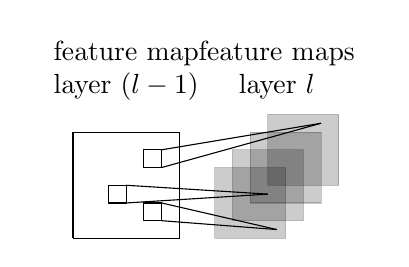
\begin{tikzpicture}[scale=0.45]
		    \node at (1.5,4.75){\begin{tabular}{c}feature map\\layer $(l - 1)$\end{tabular}};
	
		    \draw (0,0) -- (3,0) -- (3,3) -- (0,3) -- (0,0);
		
		    \draw (2,2) -- (2.5,2) -- (2.5,2.5) -- (2,2.5) -- (2,2);
		    \draw (2,0.5) -- (2.5,0.5) -- (2.5,1) -- (2,1) -- (2,0.5);
		    \draw (1,1) -- (1.5,1) -- (1.5,1.5) -- (1,1.5) -- (1,1);
		
		    \draw (2.5,2) -- (7,3.25);
		    \draw (2.5,2.5) -- (7,3.25);

		    \draw (2.5,1) -- (5.75,0.25);
		    \draw (2.5,0.5) -- (5.75,0.25);
		
		    \draw (1.5,1.5) -- (5.5,1.25);
		    \draw (1.5,1) -- (5.5,1.25);
		
		    \node at (5.75,4.75){\begin{tabular}{c}feature maps\\layer $l$\end{tabular}};
		
		    \draw[fill=black,opacity=0.2,draw=black] (5.5,1.5) -- (7.5,1.5) -- (7.5,3.5) -- (5.5,3.5) -- (5.5,1.5);
		    \draw[fill=black,opacity=0.2,draw=black] (5,1) -- (7,1) -- (7,3) -- (5,3) -- (5,1);
		    \draw[fill=black,opacity=0.2,draw=black] (4.5,0.5) -- (6.5,0.5) -- (6.5,2.5) -- (4.5,2.5) -- (4.5,0.5);
		    \draw[fill=black,opacity=0.2,draw=black] (4,0) -- (6,0) -- (6,2) -- (4,2) -- (4,0);
	    \end{tikzpicture}
	}
	\subfigure[\label{subfig:local-contrast-layer}]{
	    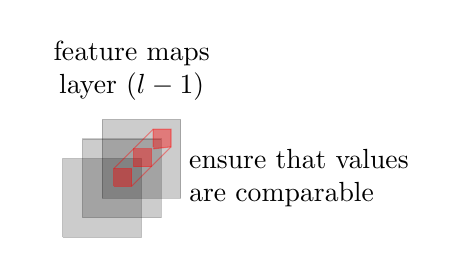
\begin{tikzpicture}[scale=0.5]
	        \node at (1.75,4.25){\begin{tabular}{c}feature maps\\layer $(l - 1)$\end{tabular}};
	        
			\draw[fill=black,opacity=0.2,draw=black] (1,1) -- (3,1) -- (3,3) -- (1,3) -- (1,1);
			\draw[fill=black,opacity=0.2,draw=black] (0.5,0.5) -- (2.5,0.5) -- (2.5,2.5) -- (0.5,2.5) -- (0.5,0.5);
			\draw[fill=black,opacity=0.2,draw=black] (0,0) -- (2,0) -- (2,2) -- (0,2) -- (0,0);
			
			\draw[opacity=0.4,draw=red,fill=red] (2.3,2.25) -- (2.75,2.3) -- (2.75,2.75) -- (2.3,2.75) -- (2.3,2.3);
			\draw[opacity=0.4,draw=red,fill=red] (1.8,1.8) -- (2.25,1.8) -- (2.25,2.25) -- (1.8,2.25) -- (1.8,1.8);
			\draw[opacity=0.4,draw=red,fill=red] (1.3,1.3) -- (1.75,1.3) -- (1.75,1.75) -- (1.3,1.75) -- (1.3,1.3);
			\draw[opacity=0.4,draw=red](1.3,1.75) --  (1.8,2.25);
			\draw[opacity=0.4,draw=red](1.75,1.3) -- (2.25,1.8);
			\draw[opacity=0.4,draw=red](2.25,1.8) -- (2.75,2.3);
			\draw[opacity=0.4,draw=red](1.8,2.25) -- (2.3,2.75);
			
			\node at (6,1.5){\begin{tabular}{l}ensure that values\\are comparable\end{tabular}};
		\end{tikzpicture}
	}
	\subfigure[\label{subfig:pooling-layer}]{
	    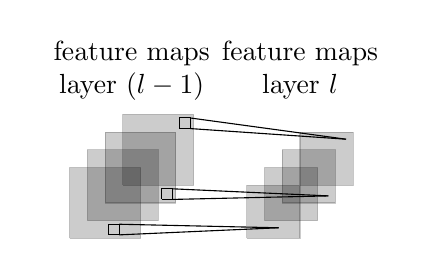
\begin{tikzpicture}[scale=0.45]
		    \node at (1.75,4.75){\begin{tabular}{c}feature maps\\layer $(l-1)$\end{tabular}};
		
		    \draw[fill=black,opacity=0.2,draw=black] (1.5,1.5) -- (3.5,1.5) -- (3.5,3.5) -- (1.5,3.5) -- (1.5,1.5);
		    \draw[fill=black,opacity=0.2,draw=black] (1,1) -- (3,1) -- (3,3) -- (1,3) -- (1,1);
		    \draw[fill=black,opacity=0.2,draw=black] (0.5,0.5) -- (2.5,0.5) -- (2.5,2.5) -- (0.5,2.5) -- (0.5,0.5);
		    \draw[fill=black,opacity=0.2,draw=black] (0,0) -- (2,0) -- (2,2) -- (0,2) -- (0,0);
		
		    \draw (3.1,3.1) -- (3.4,3.1) -- (3.4,3.4) -- (3.1,3.4) -- (3.1,3.1);
		    \draw (2.6,1.1) -- (2.9,1.1) -- (2.9,1.4) -- (2.6,1.4) -- (2.6,1.1);
		    \draw (1.1,0.1) -- (1.4,0.1) -- (1.4,0.4) -- (1.1,0.4) -- (1.1,0.1);
		
		    \draw (3.4,3.4) -- (7.8,2.8);
		    \draw (3.4,3.1) -- (7.8,2.8);
		
		    \draw (2.9,1.4) -- (7.3,1.2);
		    \draw (2.9,1.1) -- (7.3,1.2);
		
		    \draw (1.4,0.4) -- (5.9,0.3);
		    \draw (1.4,0.1) -- (5.9,0.3);
		
		    \node at (6.5,4.75){\begin{tabular}{c}feature maps\\layer $l$\end{tabular}};
		
		    \draw[fill=black,opacity=0.2,draw=black] (6.5,1.5) -- (8,1.5) -- (8,3) -- (6.5,3) -- (6.5,1.5);
		    \draw[fill=black,opacity=0.2,draw=black] (6,1) -- (7.5,1) -- (7.5,2.5) -- (6,2.5) -- (6,1);
		    \draw[fill=black,opacity=0.2,draw=black] (5.5,0.5) -- (7,0.5) -- (7,2) -- (5.5,2) -- (5.5,0.5);
		    \draw[fill=black,opacity=0.2,draw=black] (5,0) -- (6.5,0) -- (6.5,1.5) -- (5,1.5) -- (5,0);
	    \end{tikzpicture}
	}
	\caption{Illustration of a \ref{subfig:convolutional-layer} convolutional layer; \ref{subfig:local-contrast-layer} local contrast normalization layer; and \ref{subfig:pooling-layer} pooling layer.}
	\label{fig:convolutional-layer}
\end{figure}

\subsubsection{Pooling Layer}
\label{subsubsec:pooling-layer}

While LeCun \etal \cite{LeCunBoserDenkerhendersonHowardHubbardJackel:1989} use subsampling within convolutional layers (that is, the convolution in Equation \eqref{eq:convolutional-layer} is not applied on every entry of the input feature maps), recent architectures prefer to use separate pooling layers to reduce the size of the feature maps and introduce invariance to noise and distortions. Similar to the aggregation step of local descriptors used by Ge \etal \cite{GeKeSun:2013}, max pooling or average pooling are common:
\vspace{-6px}
\begin{description}
	\item[Average pooling] computes the average value within (non-overlapping) windows; while
	\vspace{-14px}
	\item[Max pooling] computes the maximum value within (non-overlapping) windows.
\end{description}
\vspace{-6px}
Pooling has been found to improve convergence and reduce overfitting \cite{KrizhevskySutskeverHinton:2012}. Note that pooling can also be used with overlapping filters, see \cite{KrizhevskySutskeverHinton:2012}.

\subsubsection{Fully-Connected Layer}
\label{subsubsec:fully-connected}

If layer $l$ is a fully connected layer and layer $(l - 1)$ one of the above layers, the input feature maps $Y_i^{(l-1)}$ are interpreted as $m_2^{(l-1)} \cdot m_3^{(l-1)}$-dimensional vectors and layer $l$ computes:
\begin{align}
    y_i^{(l)} = f\left(z_i^{(l)}\right) = f\left(\sum_{j = 1}^{m_1^{(l-1)}} \sum_{r = 1}^{m_2^{(l-1)}} \sum_{s = 1}^{m_3^{(l-1)}} w_{i,j,r,s}^{(l)} \left(Y_j^{(l-1)}\right)_{r,s}\right),\quad \forall 1 \leq i \leq m^{(l)}\label{eq:fully-connected}.
\end{align}
Note that, in contrast to convolutional layers, this layer already includes non-linearities. In the case that layer $(l-1)$ is a fully connected layer, Equation \eqref{eq:fully-connected} can be applied analogously to Equation \eqref{eq:neural-network}.
%\begin{align}
%    y_i^{(l)} = f\left( \sum_{j = 1}^{m^{(l-1)}} w^{(l)}_{i,j} y_j^{(l - 1)} + w^{(l)}_{i,0}\right),\quad 1 \leq i \leq m_1^{(l)}\label{eq:fully-connected-simple}.
%\end{align}
In convolutional neural networks, both layer $(L - 1)$ and layer $L$ are usually fully connected layers and layer $L$ uses the softmax activation function and is used for classification.

\subsection{Architectures}
\label{subsec:architectures}

Most architectures used in practice can be described using the layer types discussed above (for example \cite{LeCunBoserDenkerhendersonHowardHubbardJackel:1989,JarrettKavukcuogluRanzatoLeCun:2009}). For example, the architecture introduced by Krizhevsky \etal can be described as follows. Five convolutional layers with rectified linear unit non-linearity layers are followed by three fully connected layers
\footnote{
    The exact architecture can also be seen when consulting the reference model shipped with Caffe \cite{JiaShelhamerDonahueKarayevLongGirshickGuadarramaDarrell:2014}, see Section \ref{sec:implementations}. Note that Caffe requires some extra layer types for training as well as pre-processing and includes dropout regularization, discussed in Section \ref{subsubsec:regularization}, as additional layer type.
}.
Local contrast normalizaton layers are used after the first and second non-linearity layers (corresponding to the first and second convolutional layers). Overlapping max pooling layers are used after the first and second contrast normalization layer as well as after the fifth non-linearity layer. Although not formalized in Section \ref{subsubsec:convolutional-layer}, the convolutional layers are not necessarily fully connected to the previous layers, that is the sum in Equation \eqref{eq:convolutional-layer} does not run over all input feature maps. This is due to computational reasons, see \cite{KrizhevskySutskeverHinton:2012}. The last layer uses softmax activation functions. Figure \ref{fig:architecture} shows the overall architecture including the specific fiilter and feature map sizes.
% Overall, these are $18$ layers with $y^{(18)}$ being the posterior probabilities and $y^{(17)}$, $y^{(16)}$ the previous fully connected layers.
\begin{figure}
	\centering
	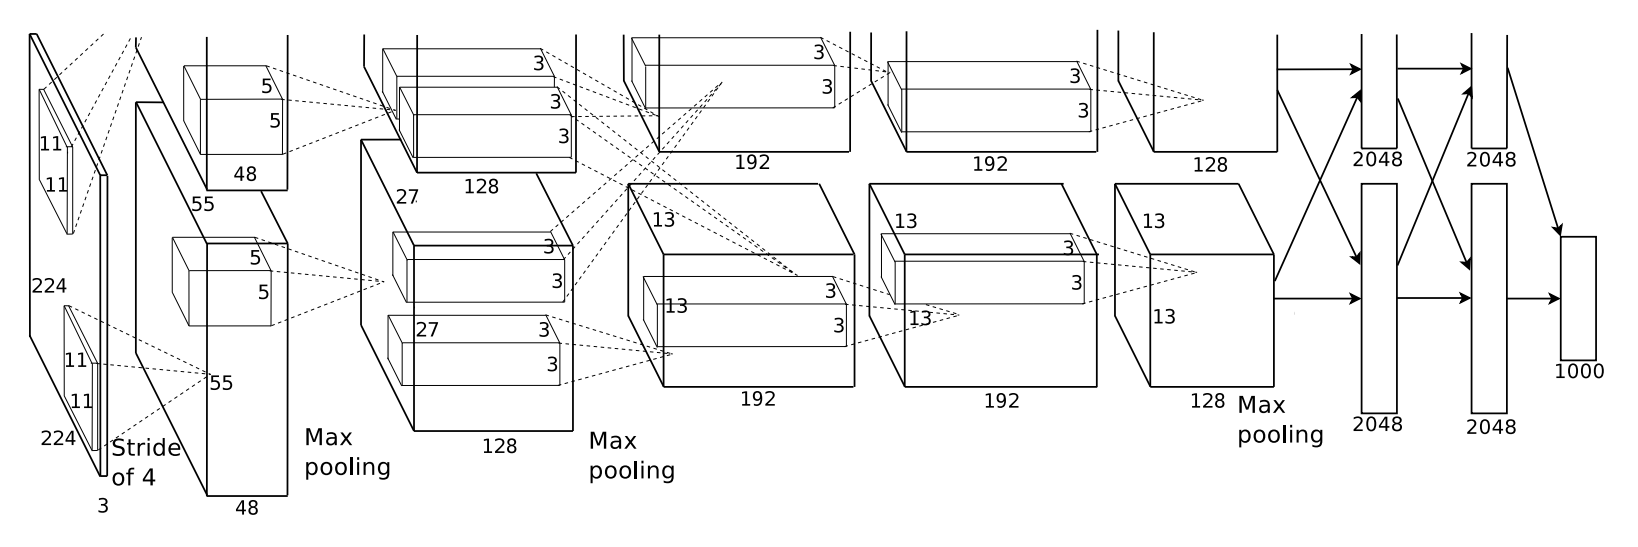
\includegraphics[scale=0.4]{pictures/architecture}
	\caption{The architecture used by Krizhevsky \etal \cite{KrizhevskySutskeverHinton:2012}. The number $m_1^{(l)}$ of computed feature maps in layer $l$ is indicated by the width of the corresponding cuboid, while the size $m_2^{(l)} \times m_3^{(l)}$ of the feature maps is indicated by the height and depth, respectively. In addition, the size of the filters $W_{i,j}^{(l)}$ is shown. For example, the input is given by a single gray-scale image of size $244 \times 244$. Using filters of size $11 \times 11$, the first convolutional layer computes $96 = 48 + 48$ feature maps of size $55 \times 55$. Furthermore, the filters in the first convolutional layer are applied in strides of $4$ pixels. We note that the architecture has been parallelized and refer to \cite{KrizhevskySutskeverHinton:2012} for details.}
	\label{fig:architecture}
\end{figure}

\subsection{Available Implementations}
\label{sec:implementations}

The main problem of implementing and training deep convolutional neural networks is computational efficiency. Therefore, most implementations use one or more GPUs. For example, the original implementation by Krizhevsky \etal uses two Nvidida GTX 580
\footnote{
    The implementation is available at \url{http://www.cs.toronto.edu/~kriz/}.
} -- still, training on the ImageNet dataset \cite{DengDongSocherLiLiLi:2009} took several days. As a result, pre-trained models have become quite popular (that is, the weights of a trained network together with a specification of the network architecture are shared with the community).
This is simplified by publicly available frameworks as for example Caffe \cite{JiaShelhamerDonahueKarayevLongGirshickGuadarramaDarrell:2014}, which comes with several pre-trained models using different architectures.
Another popular convolutional neural network library is OverFeat
\footnote{
    Available at \url{http://cilvr.nyu.edu/doku.php?id=code:start}.
}.
% Further, since the success by Krizhevsky \etal \cite{KrizhevskySutskeverHinton:2012}, frameworks for deep learning on various platforms and using different programming languages (for example Mocha, written in Julia
% \footnote{
    % Mocha is a deep learning framework for Julia, a young (2012) programming language designed for scientific computing. See \url{https://github.com/pluskid/Mocha.jl}.
% }) have been created and are gaining popularity across the borders of computer vision
% \footnote{
    % We refer to \url{http://deeplearning.net/software_links/} for a complete list of available implementations.
% }.

\subsection{Training}
\label{subsec:training}

Training convolutional neural networks means to adjust the weights $\mathbf{W} = \{w_{i,j,r,s}^{(l)}\}$ according to a loss applied on layer $L$. Given a training set $\{(x_1,t_1),\ldots,(x_N,t_N)\}$ with $t_n \in \{1,\ldots,m^{(L)}\}$ being class labels, common loss functions for classification include the sum-of-squared error and the cross-entropy error.
Instead, Krizhevsky \etal minimize the multinomial logistic loss:
\begin{align}
    E(\mathbf{W}) = - \frac{1}{m^{(L)}} \sum_{n = 1}^{N} log\left(y_{t_n}^{(L)}\right)\label{eq:multinomial-loss}
\end{align}
where $y_{t_n}^{(L)}$ is expected to model the posterior probability $p(t_n | x_n)$ of sample $x_n$ belonging to class $t_n$. These loss functions can be defined on the whole training set, as in Equation \eqref{eq:multinomial-loss}, on so-called mini-batches, that is on small subsets of the training set, or on individual training examples. Therefore, convolutional neural networks can also be trained online.

A common algorithm used for minimization is gradient descent, an iterative technique which, starting with an initial guess $\mathbf{W}[0]$, iteratively takes steps in the direction of the negative gradient (that is, the direction of the steepest descent in $L_2$ norm). Following \cite{Bottou:2012}, and given a learning rate $\gamma$, gradient descent is implemented using the update step
\begin{align}
    \mathbf{W}[\tau + 1] = \mathbf{W}[\tau] - \gamma \nabla E\left(\mathbf{W}[\tau]\right)\label{eq:gradient-descent}.
\end{align}
The chosen learning rate $\gamma$ is crucial and usually has strong influence on the found minima. A widely used extension is gradient descent with momentum term which aims to avoid oscillation while using a high learning rate for fast training. The update step changes to:
\begin{align}
    \mathbf{W}[\tau + 1] = \mathbf{W}[\tau] - \gamma \nabla E\left(\mathbf{W}[\tau]\right) + \nu(\mathbf{W}[\tau] - \mathbf{W}[\tau - 1])
\end{align}
where $\nu$ is the momentum parameter.
% In practice, the learning rate may be depending on the iteration (that is, manually or automatically adapted during the training process).

Stochastic gradient descent applies the update of Equation \eqref{eq:gradient-descent} on a subset of randomly selected samples. It can be shown that stochastic gradient descent converges under relatively loose conditions \cite{Bottou:2012}. In addition, stochastic gradient descent may be beneficial for large-scale learning \cite{Bottou:2012} and improve the generalization performance of the learned model \cite{BottouBousquet:2007}. 
% Krizhevsky \etal \cite{KrizhevskySutskeverHinton:2012} additionally use weight decay, see Section \ref{subsubsec:regularization}.

For applying stochastic gradient descent, the gradient $\nabla E(\mathbf{W}[\tau])$ needs to be computed in each iteration. Therefore, Error Backpropagation has been proposed and allows to compute the gradient $\nabla E(\mathbf{W}[\tau])$ in~$\mathcal{O}\left(|\mathbf{W}|\right)$ \cite{Bishop:1995}.

%\subsubsection{Deep Training}
%\label{subsubsec:deep-training}

\subsubsection{Regularization}
\label{subsubsec:regularization}

Regularization is used to control the complexity of the model during training to prevent overfitting. For example, Krizhevsky \etal use weight decay and dropout as regularization during training. Weight decay is simple $L_2$-normalization of the weights and used because large weights result in poor generalization~\cite{Bishop:1995}. The updated loss function can be written as:
\begin{align}
    \hat{E}(\mathbf{W}) = E(\mathbf{W}) + \lambda \|\mathbf{W}\|_2.
\end{align}
In contrast, dropout \cite{KrizhevskySutskeverHinton:2012} tries to decouple pairs of computation units (that is individual elements within the feature maps $Y_i^{(l)}$ or the computed vectors $y^{(l)}$). Each such unit is deactivated (that is, set to zero) with probability one half. The intention is to avoid subsequent layers or neighboring units being dependent on specific units.
